
\section{Results}\label{sec:results}

Now that we have different clustering results obtained from PAM, NEMO, and Spectral clustering, along with different choices of matrix integration for PAM, we can proceed with comparing the aforementioned results with the disease subtypes reported by iCluster.

First, we will compute the evaluation metrics RI, ARI, and NMI for all the clustering algorithms proposed compared to the PAM50. Table~\ref{tab:results} highlights the different values obtained for all different metrics.

\begin{table}[!t]
    \centering
    \caption{Clustering results for different metrics}
    \begin{tabular}{|c|c|c|c|}
    \hline
    \multirow{2}{*}{Clustering} & \multicolumn{3}{c|}{Metric} \\ \cline{2-4} 
    & RI & ARI & NMI \\ \hline
    PAM\_miRNA & 0.5424122 & 0.024669347 & 0.02763638 \\
    PAM\_mRNA & 0.5574964 & 0.037660032 & 0.05320068 \\
    PAM\_protein & 0.5523704 & 0.007886092 & 0.01965598 \\
    PAM\_W\_avg & 0.5598145 & 0.023650868 & 0.04030343 \\
    PAM\_SNF & 0.6316769 & 0.179466272 & 0.15674451 \\
    PAM\_AF\_NEMO & 0.5617735 & 0.032536154 & 0.05438288 \\
    NEMO & 0.3803056 & 0.014593726 & 0.06891715 \\
    Spectral & 0.6051326 & 0.119098119 & 0.11723454 \\ \hline
    \end{tabular}
    \label{tab:results}
\end{table}

With the evaluation metric values available, we proceed to visualize the results in  Fig.~\ref{fig:clustering} and Fig.~\ref{fig:evaluation}.

\begin{figure}[!t]
    \centerline{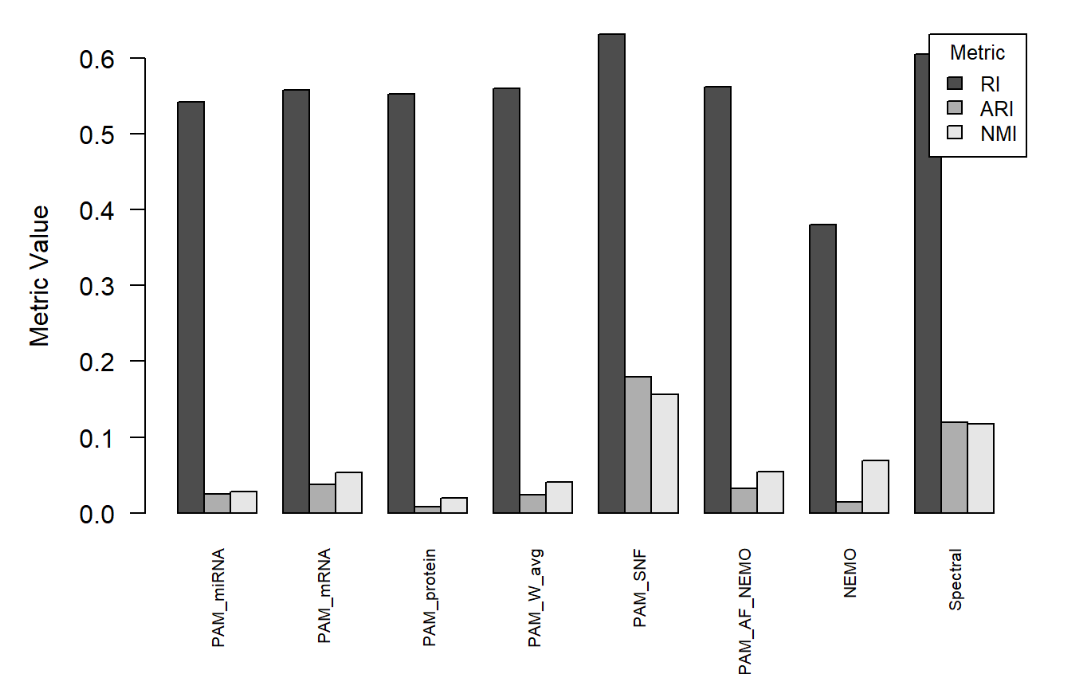
\includegraphics[width=\columnwidth]{images/clustering.png}}
    \caption{Performance of Clustering Techniques (by clustering method)}
    \label{fig:clustering}
\end{figure}

\begin{figure}[!t]
    \centerline{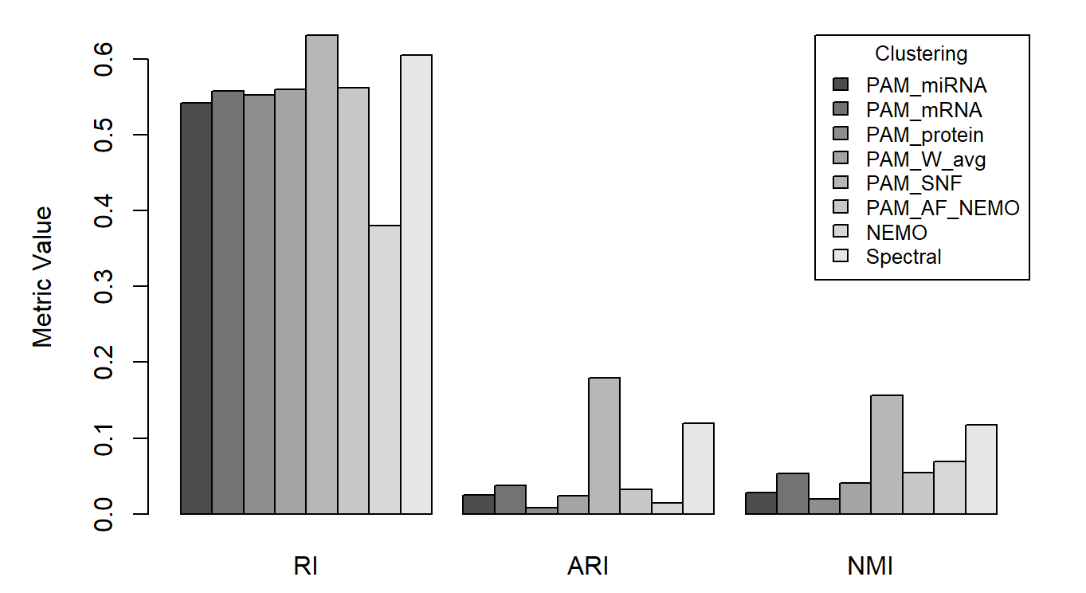
\includegraphics[width=\columnwidth]{images/evalutation.png}}
    \caption{Performance of Clustering Techniques (by evaluation metric)}
    \label{fig:evaluation}
\end{figure}

Analyzing the results of clustering algorithms compared to PAM50, the following observations can be made:

\begin{itemize}[\IEEEsetlabelwidth{Z}]
    \item Overall, it can be seen that performing the PAM algorithm on the SNF integrated matrix has the best performance among the techniques explored, followed by the Spectral clustering approach on the same integrated matrix, which also provides promising results.
    \item It is evident that the RI metric provides more optimistic results, so it would be a valid idea to present other measures such as ARI (based on counting pairs) and NMI (based on information theory) to better interpret the results.
    \item Due to the simplicity of the chosen preprocessing techniques (such as selecting the first 100 highest variance, or selecting only the samples having all the 3 data sources available instead of imputing), it is probable that some of the aforementioned group of genes are removed. This could potentially complicate the identification of subgroups based on alternative features and result in poor performance.
    \item PAM50 solely relies on mRNA data from different genes, whereas our clustering approach integrates multiple data sources from three distinct omics. Consequently, we have a richer dataset for clustering analysis, potentially resulting in clusters with unique biological interpretations that differ from the ones reported by PAM50.
\end{itemize}
